\documentclass[conference]{IEEEtran}
\usepackage{cite,tikz,balance}
\usepackage{amsmath,amssymb,amsfonts,booktabs,graphicx,textcomp,xcolor}
\usepackage[hidelinks]{hyperref}
\usetikzlibrary{arrows.meta,positioning,calc}
% All tables span exactly one IEEE column with shared typography.
\newcommand{\papertablestyle}{\centering\small\setlength{\tabcolsep}{3pt}\renewcommand{\arraystretch}{1.05}}
\newcommand{\E}{\mathbb E}
% Natural two-column flow; retain standard IEEEtran typography.
% IEEE template: https://www.overleaf.com/latex/templates/ieee-conference-template/grfzhhncsfqn
% Preserve IEEEtran margins, columns, fonts and spacing.
% Compile from TPEC_conference using the independent conference_refs.bib.
\title{Informative Power-System Probing via
Sequential Bayesian Experimental Design}
% For two authors, remove the final \and and third author block.
\author{\IEEEauthorblockN{First Author}
\IEEEauthorblockA{\textit{Department / Institution}\\
City, Country\\
email@example.com}
\and
\IEEEauthorblockN{Second Author}
\IEEEauthorblockA{\textit{Department / Institution}\\
City, Country\\
email@example.com}
\and
\IEEEauthorblockN{Third Author}
\IEEEauthorblockA{\textit{Department / Institution}\\
City, Country\\
email@example.com}}
\begin{document}
\raggedbottom
\maketitle
\begin{abstract}
Power-grid stability is vital to industrial operations and daily life.
Understanding latent parameters, including inertia $M$ and effective frequency
response $K$, helps predict disturbance responses and inform stability control.
Active probing reduces parameter uncertainty through small injected signals
and measured responses. However, selecting all probes in advance prevents
adaptation to new measurements, while optimizing one probe at a time incurs
substantial online computation and overlooks future information gains.
We apply adaptive sequential Bayesian optimal experimental design to address
these limitations by selecting probe durations from accumulated observations
while accounting for the information obtainable from the remaining probes.
On reduced IEEE9 and IEEE14 models, we compare DAD, RL-sBOED, and Step-DAD
with Myopic, an optimized fixed sequence, and random probing. All three
learned methods achieve higher estimated expected information gain than the
baselines. DAD and RL-sBOED also substantially reduce online decision time
relative to Myopic by learning adaptive policies offline.
\end{abstract}
\begin{IEEEkeywords}
Bayesian experimental design, power-system identification, adaptive probing,
expected information gain, rate of change of frequency.
\end{IEEEkeywords}

\section{Introduction}
Stable power-system operation supports reliable electricity supply.
Engineers need information about inertia $M$ and effective frequency
response $K$ to predict disturbance responses and choose operating
and control actions. Reducing uncertainty in these parameters can support better
informed decisions. Active probing identifies them by injecting controlled
signals and measuring frequency responses~\cite{peng2024probing}.

The information obtained depends on the probing inputs. Our aim is to
learn more about $M$ and $K$ with the same number of experiments by
adapting successive probes to observed responses. Sequential Bayesian
optimal experimental design (sBOED) provides the framework. Fixed designs
cannot use new observations; myopic designs use them but optimize only
the next experiment~\cite{huan2016sequential}. Full-sequence design can
account for how each probe informs later choices. It must also account
for the grid's physical state changes caused by preceding probes.

Existing methods offer different information--computation trade-offs.
Deep adaptive design (DAD) learns a policy offline to maximize information
over a complete sequence~\cite{foster2021dad}. RL-sBOED learns policies
through simulated rewards~\cite{blau2022rlsboed}; Step-DAD refines a
pretrained policy after observations arrive~\cite{hedman2025stepdad}.
We evaluate whether these methods yield more information under matched
grid probing constraints, and whether online refinement justifies its cost.

We formulate continuous probe-duration selection with a shared sensor
model and physical state carried between experiments. Six existing methods are compared on reduced IEEE9 and
IEEE14 systems at equal probe budgets. We report EIG, seed variability, and offline and online computation. Our
contribution is the power-system design formulation and matched evaluation;
the policy algorithms are existing methods, and conclusions are limited
to the stated models and sensor.

\section{Problem Formulation}\label{sec:problem}
We seek to reduce uncertainty in $M$ and $K$ through informative probes
within a budget of $T$ design steps.
Here $t=1,\ldots,T$ indexes design steps, $d$ denotes
elapsed time within each probe window, and $D_t$ is the selected
pulse duration.

\subsection{Unknown Parameters and Power-System Model}
For a reduced network with $m$ machines, the unknown parameter vector is
$\theta=(M_1,\ldots,M_m,K_1,\ldots,K_m)$, where $M_i$ and $K_i$
are inertia and effective frequency-response coefficients. The prior
$p_0(\theta)$ has independent components
$M_i\sim\mathcal U(0.7\bar M_i,1.3\bar M_i)$ and
$K_i\sim\mathcal U(0.1\bar K_i,\bar K_i)$.
One draw of $\theta$ remains fixed throughout all $T$ probes.

Let $\delta_i$ be rotor angle, $\omega_i$ angular-speed deviation,
and $u_i$ the applied probing power. The reduced swing model is
\begin{equation}
\begin{aligned}
\dot\delta_i &= \omega_i,\\
M_i\dot\omega_i
 &= u_i-\left(D_i+\frac{K_i}{2\pi}\right)\omega_i\\
 &\quad-\sum_{j=1}^{m}B_{ij}\sin(\delta_i-\delta_j).
\end{aligned}
\label{eq:swing}
\end{equation}
Dots denote derivatives with respect to physical time $d$. The damping $D_i$ and network
couplings $B_{ij}$ are known; frequency deviation is
$\Delta f_i=\omega_i/(2\pi)$ in Hz. The units of $M_i$, $K_i$ and
$D_i$ are pu$\,\mathrm{s}^2$/rad, pu/Hz and pu$\,\mathrm{s}$/rad,
respectively, on a 100-MVA base at nominal frequency 60 Hz.
All angles and speed deviations start at zero. Net mechanical injections
are zero in this deviation model, making the initial unforced state an
equilibrium.

IEEE9 retains buses 1, 2 and 3; IEEE14 retains buses 1, 2, 3, 6 and 8.
Test-case reactances~\cite{zimmerman2011matpower} define a lossless
Laplacian $\mathbf L$. Eliminating algebraic buses $l$ while retaining
machines $g$ gives
$\mathbf L_{\mathrm{red}}=\mathbf L_{gg}-\mathbf L_{gl}\mathbf L_{ll}^{-1}\mathbf L_{lg}$,
with $B_{ij}=-(\mathbf L_{\mathrm{red}})_{ij}$ for $i\ne j$ and $B_{ii}=0$.
Resistance, voltage dynamics and transformer tap effects are omitted.
Table~\ref{tab:physical} summarizes the model parameterization.
Nominal inertia is computed as $\bar M_i=2H_i/(2\pi f_0)$, with
$f_0=60$ Hz. For IEEE9, $H=(23.64,6.40,3.01)$ s matches published
machine data~\cite[Table~2]{kaur2016transient}. For IEEE14,
$H=(4,6.5,5,5,5)$ s is prescribed at buses $(1,2,3,6,8)$ as a
benchmark setting, without a verified literature source for these values.
For both networks, $\bar K_i=K_{\mathrm{tot}}w_i$, with
$K_{\mathrm{tot}}=0.5$ pu/Hz. The allocation weights are
$w=(0.5875,0.2625,0.15)$ for IEEE9 and
$w=(8,13,10,10,10)/51$ for IEEE14. Fixed damping satisfies
$D_i=(0.1\,\mathrm{s}^{-1})\bar M_i$.
The response scales, damping and prior ranges are shared study assumptions,
not validated operating-grid parameters. Table entries are rounded;
configurations retain full precision. Training and evaluation draw
independently from the same prior.
\begin{table}[t]
\caption{Prior scales and damping coefficients}
\label{tab:physical}
\papertablestyle
\begin{tabular*}{\columnwidth}{@{\extracolsep{\fill}}llrrr@{}}
\toprule Network & Bus & $\bar M_i$ & $\bar K_i$ & $D_i$\\\midrule
IEEE9 & 1 & 0.1254141 & 0.2937500 & 0.0125414\\
 & 2 & 0.0339531 & 0.1312500 & 0.0033953\\
 & 3 & 0.0159685 & 0.0750000 & 0.0015969\\
IEEE14 & 1 & 0.0212207 & 0.0784314 & 0.0021221\\
 & 2 & 0.0344836 & 0.1274510 & 0.0034484\\
 & 3, 6, 8 & 0.0265257 & 0.0980392 & 0.0026526\\
\bottomrule
\end{tabular*}
\end{table}

\subsection{Probe Design and Observation Model}
The probe design is $\xi_t=(A_t,B_t,D_t)$: amplitude,
injection bus and pulse duration. This study fixes $A_t=0.05$ pu
and $B_t=1$; only $D_t$ is optimized. The raised-cosine input for
$0\le d\le D_t$ is
\begin{equation}
u_{B_t,t}(d)
 =\frac{A_t}{2}\bigl[1-\cos(2\pi d/D_t)\bigr].
\label{eq:probe}
\end{equation}
The input is zero for $D_t<d\le D_{\mathrm{obs}}$
and at all other buses. The observation window is $D_{\mathrm{obs}}=3.5$ s. The full angle and speed state at its end becomes the initial
state of the next window, without resetting the system. Consequently,
the response depends on the complete design sequence
$\xi_{1:t}=(\xi_1,\ldots,\xi_t)$.

Write $\Delta f_{1,t}(d;\theta,\xi_{1:t})$ for the resulting bus-1
frequency deviation. The noise-free response is the signed endpoint
rate of change of frequency (RoCoF), denoted by $y_t$:
\begin{equation}
y_t(\theta,\xi_{1:t})=
\frac{\Delta f_{1,t}(D_{\mathrm{obs}})-\Delta f_{1,t}(D_{\mathrm{obs}}-\Delta d_{\mathrm{samp}})}{\Delta d_{\mathrm{samp}}}.
\label{eq:sensor}
\end{equation}
The frequency arguments $\theta,\xi_{1:t}$ are suppressed in the
numerator. With sampling interval $\Delta d_{\mathrm{samp}}=0.025$ s, the measured
response follows
\begin{equation}
y_{\mathrm{obs},t}=y_t(\theta,\xi_{1:t})+\epsilon_t,
\qquad \epsilon_t\sim\mathcal N(0,\sigma^2),
\label{eq:noise}
\end{equation}
where $\sigma=0.005$ Hz/s and noise is independent across windows.
Each observation becomes available at window end. Decision latency is
idealized as zero in simulated time.

\subsection{Sequential Decisions and Bayesian Updating}
The observation model connects the physical experiment to inference and
subsequent decisions. The data after step $t$ are the ordered design--observation
history $h_t=((\xi_k,y_{\mathrm{obs},k}))_{k=1}^{t}$, with $h_0=\varnothing$.
A policy $\pi$ selects $\xi_t$ using only observed history $h_{t-1}$,
with amplitude and bus fixed as above. It has no access to true parameters
or physical state. Feasible durations satisfy
\begin{equation}
\begin{aligned}
0.2&\le D_t\le3, &&t=1,\ldots,T,\\
D_t-D_{t-1}&\ge \Delta D_{\min}, &&t=2,\ldots,T,
\end{aligned}
\label{eq:bounds}
\end{equation}
where $\Delta D_{\min}=0.01$ s. At step $t$, the upper limit is tightened to
$3-(T-t)\Delta D_{\min}$ to leave room for the remaining probes; the lower
limit is $0.2$ initially and $D_{t-1}+\Delta D_{\min}$ thereafter.
All methods map a unit action into this interval without sorting or
discretizing durations. Let $\Pi$ denote the policies satisfying these constraints;
any policy randomness is independent of $\theta$.

The observation model defines a Gaussian likelihood
$p(y_{\mathrm{obs},t}\mid\theta,h_{t-1},\xi_t)$ with mean
$y_t(\theta,\xi_{1:t})$ and variance $\sigma^2$.
Bayes' rule updates parameter uncertainty after each measurement:
\begin{equation}
p(\theta\mid h_t)=
\frac{p(y_{\mathrm{obs},t}\mid\theta,h_{t-1},\xi_t)\,p(\theta\mid h_{t-1})}
{p(y_{\mathrm{obs},t}\mid h_{t-1},\xi_t)}.
\label{eq:posterior}
\end{equation}
The denominator is the predictive density, obtained by integrating the
numerator over $\theta$, and $p(\theta\mid h_0)=p_0(\theta)$.
Each candidate parameter vector propagates its own physical state under
the observed designs to evaluate the likelihood. Conditional on the
history, design selection provides no additional knowledge of $\theta$;
policy probabilities therefore cancel from the Bayesian update.

\subsection{Expected Information Gain and Design Objective}
To compare possible design policies, we quantify the uncertainty reduction
produced by their observations using the Kullback--Leibler divergence
of the terminal posterior from the prior.
The expected information gain (EIG) of policy $\pi$ is
\begin{equation}
\mathcal I_T(\pi)=\E_{h_T\mid\pi}
\!\left[D_{\mathrm{KL}}\bigl(p(\theta\mid h_T)\,\|\,p_0(\theta)\bigr)\right].
\label{eq:eig}
\end{equation}
Here $D_{\mathrm{KL}}(p\|q)=\int p(\theta)\log[p(\theta)/q(\theta)]\,d\theta$;
natural logarithms express information in nats. The expectation averages
over parameter draws, measurement noise and any policy randomness.
The sequential Bayesian design problem is
\begin{equation}
\pi^\star\in\operatorname*{arg\,max}_{\pi\in\Pi}\mathcal I_T(\pi).
\label{eq:design_problem}
\end{equation}
Thus all methods receive the same number of probes and seek greater
expected reduction in parameter uncertainty. Offline and online
computation are measured separately from this information objective.

Exact EIG requires intractable marginal likelihoods. We use the sequential
prior-contrastive (sPCE) lower bound~\cite{foster2021dad} for training and
evaluation. Let $\theta^{(0)}\sim p_0$ generate the observed history and
let $\theta^{(1)},\ldots,\theta^{(L)}$ be independent prior contrasts.
For any candidate $\theta$, define the observation likelihood along the
realized sequence as
\begin{equation}
\mathcal L_t(\theta)=\prod_{k=1}^{t}
p(y_{\mathrm{obs},k}\mid\theta,h_{k-1},\xi_k).
\label{eq:likelihood}
\end{equation}
The sampled information score is then
\begin{equation}
\widehat I_t=\log\frac{\mathcal L_t(\theta^{(0)})}
{\frac{1}{L+1}\sum_{\ell=0}^{L}\mathcal L_t(\theta^{(\ell)})}.
\label{eq:spce}
\end{equation}
Likelihoods are evaluated in the log domain. Averaging $\widehat I_T$
over simulated sequences estimates a lower bound on $\mathcal I_T(\pi)$;
For IEEE9 and IEEE14, reported EIG values are estimated using this sPCE
lower bound; they are not exact EIG values. Individual scores can be negative but
cannot exceed $\log(L+1)$. With $L=128$, this ceiling is 4.8598 nats,
so near-ceiling scores can conceal differences in true EIG.
The generating parameter is used only by the evaluator, never supplied
to an online planner.

\section{Compared Design Methods}
The objective in~\eqref{eq:design_problem} motivates three comparisons:
optimized versus random probing, adaptive versus fixed designs, and
offline policy learning versus online optimization. The six existing
methods below select $\xi_t=(0.05,1,D_t)$ using the same feasible
duration interval~\eqref{eq:bounds} and observation model.
Table~\ref{tab:methods} distinguishes adaptation to observations from
myopic optimization of only the next probe. Fixed optimizes the full
sequence without observation feedback. Random optimizes no information
objective, so its myopia entry is N/A.

\begin{table}[t]
\caption{Comparison of experimental design methods}
\label{tab:methods}\papertablestyle
\begin{tabular*}{\columnwidth}{@{\extracolsep{\fill}}lccc@{}}
\toprule Method & Adaptive & Myopic & Optimization\\\midrule
Random & No & N/A & None\\
Fixed~\cite{huan2016sequential} & No & No & Offline\\
Myopic~\cite{huan2016sequential} & Yes & Yes & Online\\
DAD~\cite{foster2021dad} & Yes & No & Offline\\
RL-sBOED~\cite{blau2022rlsboed} & Yes & No & Offline\\
Step-DAD~\cite{hedman2025stepdad} & Yes & No & Both\\
\bottomrule\end{tabular*}
\end{table}




\subsection{Nonadaptive Designs: Random and Fixed}
Random draws $z_t\sim\mathcal U(0,1)$ independently at each step and
sets $D_t=D_t^{\min}+(D_t^{\max}-D_t^{\min})z_t$.
Here $D_1^{\min}=0.2$, $D_t^{\min}=D_{t-1}+\Delta D_{\min}$ for $t>1$,
and $D_t^{\max}=3-(T-t)\Delta D_{\min}$. Thus sampling is uniform within
the remaining feasible interval, not over complete ordered sequences.
It ignores observations and requires no offline training.

Fixed is a static Bayesian design: all durations are optimized jointly
before observations are collected~\cite[Sec.~2.4]{huan2016sequential}.
Our implementation optimizes the ordered sequence using EIG for the full sequence.
It compares short, central, long and spread interior initializations
using validation, then optimizes the selected initialization. Each
training seed yields a separately fitted sequence. During evaluation,
Fixed executes that sequence without adapting to observations.

\subsection{Online One-Step Design: Myopic}
Unlike Fixed, Myopic uses observation feedback. It follows one-step
adaptive BOED, maximizing the expected
information from the next observation under the current
posterior~\cite[Sec.~2.4]{huan2016sequential}. Our implementation maintains
a weighted particle approximation to this posterior. Before each decision after the first, particles propagate
their own states under the preceding duration and update likelihood
weights using the latest observation. Continuous search then maximizes
expected information from the next probe only, using 16 proposals,
three search rounds and 32 simulated observations per proposal.
Candidate durations obey the same constraints as all other methods.
No offline policy is trained.

\subsection{Offline-Trained Adaptive Policies: DAD and RL-sBOED}
DAD and RL-sBOED retain observation feedback while optimizing over
the full sequence offline. Both policies receive the stage index and
ordered slots containing past
durations, scaled observations and availability masks; future slots are
masked. They do not receive true parameters or physical states.
At evaluation, a forward pass produces the action without online
optimization or an explicit particle-posterior update.

DAD~\cite{foster2021dad} uses a deterministic two-layer, 64-unit tanh network, a trainable
stage bias and a sigmoid action map. Offline training maximizes EIG by differentiating through the complete simulated sequence,
including observations and carried states. In the joint Fixed/DAD
campaign, validation selects between random and interior Fixed-based
initialization. The reported DAD stage timer excludes the preceding
Fixed training; the full workflow incurs both costs.

RL-sBOED~\cite{blau2022rlsboed} uses a REDQ-style actor--critic adaptation with ten critics
and five replay updates per trajectory batch. The actor has two
128-unit ReLU layers. Its per-step information rewards are
$R_t=\widehat I_t-\widehat I_{t-1}$, with $\widehat I_0=0$ and
discount $\gamma=1$, so their sum estimates full-sequence EIG. Training therefore
accounts for future design steps without differentiating through the
simulator. Entropy regularization uses normalized tanh actions and
target entropy $-1$; reported information scores exclude entropy bonuses.
Evaluation uses the actor's deterministic output.

\subsection{Online Policy Refinement: Step-DAD}
Step-DAD~\cite{hedman2025stepdad} tests whether adapting policy weights
to the observed history improves on offline training alone. Each episode begins with the matching selected DAD checkpoint
and uses it unchanged for the first probe. Before each subsequent
decision, it assimilates the latest observation into its 128-particle
posterior. It then samples candidate parameters and their carried
states from that posterior to simulate the remaining design steps.
These future simulations condition on the actual observed history.

At each refinement, a fresh Adam optimizer performs four gradient
updates with batch size 32 and learning rate $10^{-3}$. A fixed
conditional validation batch compares the unchanged policy and all
updated candidates; the best is retained. Retained weights carry to
the next design step within the episode, but not to another episode.
The total refinement budget is $4(T-1)$ updates: 8, 12 and 16 for
$T=3,4,5$. The planner never receives the evaluator's true parameters.

For both Myopic and Step-DAD, assimilation is performed only when a
subsequent decision requires it. No final planner update is needed
after $y_{\mathrm{obs},T}$ for this EIG experiment; terminal information is computed
separately by the evaluator using~\eqref{eq:spce}.

\section{Experimental Settings}
To assess these design strategies at equal measurement budgets, we
compare all six methods at $T=3,4,5$ design steps on IEEE9 and IEEE14.
Each step applies one probe and collects one observation. The systems
share sensor and design constraints but use separate physical parameters
and trained policies.

Figure~\ref{fig:probing} connects probing to inference: observations
reweight candidate parameters through their likelihoods, and adaptive
designs use the resulting history to select later probes.

\begin{figure*}[t]
\centering
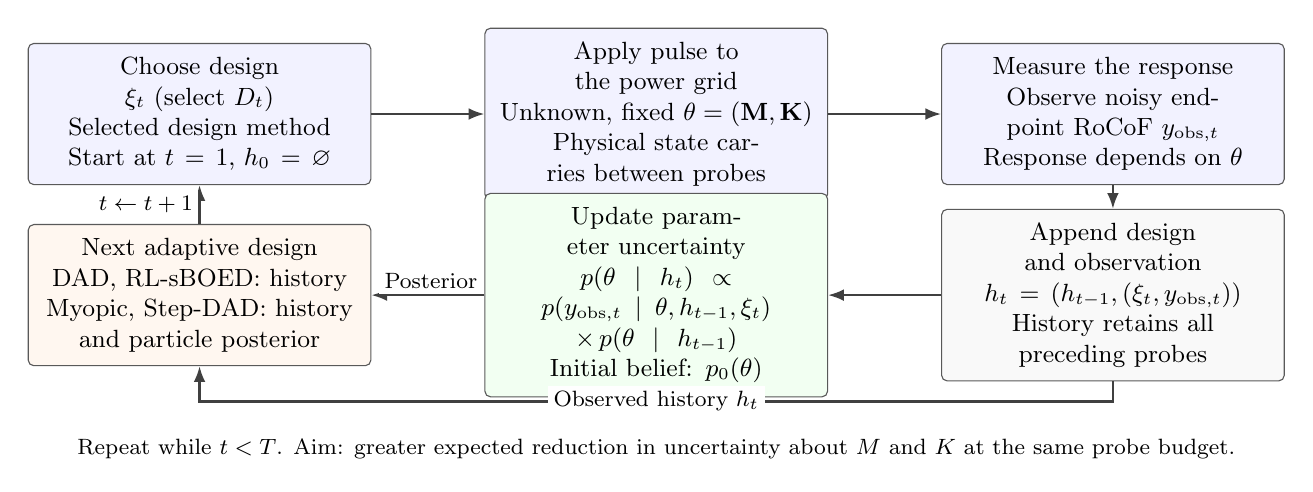
\begin{tikzpicture}[x=1cm,y=1cm,
 box/.style={draw=black!65,rounded corners=2pt,align=center,
 font=\small,inner sep=5pt,minimum height=1.15cm,text width=4.0cm},
 flow/.style={-{Latex[length=2mm]},thick,draw=black!75},
 note/.style={font=\footnotesize,align=center,fill=white,inner sep=2pt}]
\node[box,fill=blue!5] (select) at (0,0)
 {Choose design $\xi_t$ (select $D_t$)\\Selected design method\\Start at $t=1$, $h_0=\varnothing$};
\node[box,fill=blue!5] (grid) at (5.8,0)
 {Apply pulse to the power grid\\Unknown, fixed $\theta=(\mathbf M,\mathbf K)$\\Physical state carries between probes};
\node[box,fill=blue!5] (observe) at (11.6,0)
 {Measure the response\\Observe noisy endpoint RoCoF $y_{\mathrm{obs},t}$\\Response depends on $\theta$};
\node[box,fill=gray!5] (history) at (11.6,-2.3)
 {Append design and observation\\$h_t=(h_{t-1},(\xi_t,y_{\mathrm{obs},t}))$\\History retains all preceding probes};
\node[box,fill=green!5,minimum height=1.5cm] (posterior) at (5.8,-2.3)
 {Update parameter uncertainty\\$p(\theta\mid h_t)\propto$\\
 $p(y_{\mathrm{obs},t}\mid\theta,h_{t-1},\xi_t)$\\$\times\,p(\theta\mid h_{t-1})$\\Initial belief: $p_0(\theta)$};
\node[box,fill=orange!6,minimum height=1.5cm] (next) at (0,-2.3)
 {Next adaptive design\\DAD, RL-sBOED: history\\Myopic, Step-DAD: history\\and particle posterior};
\draw[flow] (select) -- (grid);
\draw[flow] (grid) -- (observe);
\draw[flow] (observe) -- (history);
\draw[flow] (history) -- (posterior);
\draw[flow] (posterior) -- node[note,above,text width=1.1cm] {Posterior} (next);
\draw[flow] (history.south) -- (11.6,-3.65)
 -- node[note,pos=.5] {Observed history $h_t$} (0,-3.65) -- (next.south);
\draw[flow] (next.north) -- node[note,left] {$t\leftarrow t+1$} (select.south);
\node[note,anchor=north] at (5.8,-4.05)
 {Repeat while $t<T$. Aim: greater expected reduction in uncertainty about $M$ and $K$ at the same probe budget.};
\end{tikzpicture}
\caption{Sequential probing and information feedback. Each response extends
the history, which determines the posterior through the likelihood.
The next adaptive design uses this history directly (DAD/RL-sBOED), or
the history and its particle posterior for online planning (Myopic/Step-DAD).
DAD/RL-sBOED do not explicitly compute a posterior. Random and Fixed use
the same physical experiment but bypass adaptive feedback. Stop after
$T$ observations; EIG is estimated separately, without requiring a
final planner update. Uncertainty reduction is expected over experiments,
not guaranteed for every observation.}
\label{fig:probing}
\end{figure*}

The swing equations are integrated by RK4 with step $1/640$ s.
Numerical state/duration Jacobians use perturbations of $10^{-5}$
and include carried-state derivatives. The verification suite compares
policy and conditional-refinement gradients with end-to-end finite
differences.

Offline training uses 2,000 updates with batch size 32 and three independent
training seeds (101, 202 and 303). The DAD and Fixed learning rate is
$10^{-3}$. Validation uses 128 systems every 100 updates. Training,
validation and evaluation use 128 contrastive samples for the sPCE
objective. Myopic and Step-DAD use 128 particles for online posterior
planning; Step-DAD performs four refinement updates after each observation
when design steps remain. Evaluation uses seeds 1001, 1002 and 1003,
with 512 simulated experimental sequences per evaluation seed.
Validation selects checkpoints without gradient updates on validation cases.
Each trained policy is evaluated on 1,536 episodes. Parameter and
measurement-noise draws are paired across methods; the online planner uses
a separate random stream. Random/Myopic have no training-seed dependence
under these streams, so identical evaluations can be shared across training
seeds. Fixed remains independently optimized for each training seed.

For trained methods, we average evaluation-seed means within each training
seed and report mean $\pm$ sample standard deviation across three trainings.
Random/Myopic report mean $\pm$ sample SD of evaluation-seed means,
not episode-level dispersion. Evaluation seed 1001 informed development and is not untouched test data.

Experiments use NVIDIA RTX 5080 and A100 GPUs, with RTX 4090 used for
development. IEEE9 offline times combine RTX 5080 and A100 runs;
online timings use RTX 5080 except Step-DAD $T=5$, training seed 303,
which ran on A100. IEEE14 timings use A100. These recorded workflow
costs do not provide a controlled runtime comparison between networks.
Configurations, source hashes and checkpoints preserve provenance.
Code: \url{https://github.com/alexschmidt123/tpec2027_power_grid}.

% Complete results under the accepted three-evaluation-seed grid protocol.
\section{Results and Discussion}
\label{sec:results}
We first compare information acquired at equal probe budgets, then examine
the computation required to obtain it. Optimization diagnostics and
estimator limitations qualify the resulting comparisons.

\subsection{Information Versus Number of Design Steps}
Tables~\ref{tab:ieee9} and~\ref{tab:ieee14} report EIG in
nats as mean $\pm$ sample SD. Trained methods use three training-seed
means; Random and Myopic use three evaluation-seed means. Both networks
use $L=128$ contrasts, giving a 4.8598-nat estimator ceiling.
\begin{table}[!ht]\caption{IEEE9 EIG}\label{tab:ieee9}\papertablestyle
\begin{tabular*}{\columnwidth}{@{\extracolsep{\fill}}lccc@{}}\toprule Method & $T=3$ & $T=4$ & $T=5$\\\midrule
Random & $0.4321\pm0.0310$ & $0.4924\pm0.0342$ & $0.5392\pm0.0471$\\
Fixed & $2.0112\pm0.0116$ & $2.3192\pm0.0004$ & $2.5066\pm0.0013$\\
Myopic & $1.9736\pm0.0438$ & $2.1707\pm0.0366$ & $2.2407\pm0.0547$\\
DAD & $2.1366\pm0.0161$ & $2.4095\pm0.0080$ & $2.6351\pm0.0179$\\
RL-sBOED & $2.1257\pm0.0027$ & $2.3963\pm0.0333$ & $2.5307\pm0.0114$\\
Step-DAD & $2.1471\pm0.0110$ & $2.4382\pm0.0048$ & $2.6621\pm0.0145$\\
\bottomrule\end{tabular*}\end{table}

\begin{table}[!ht]
\caption{IEEE14 EIG}
\label{tab:ieee14}
\papertablestyle
\begin{tabular*}{\columnwidth}{@{\extracolsep{\fill}}lccc@{}}
\toprule Method & $T=3$ & $T=4$ & $T=5$\\\midrule
Random & $0.7541\pm0.0047$ & $0.8360\pm0.0297$ & $0.8464\pm0.0252$\\
Fixed & $4.2623\pm0.0402$ & $4.4946\pm0.0345$ & $4.6624\pm0.0083$\\
Myopic & $4.2907\pm0.0368$ & $4.3990\pm0.0177$ & $4.4641\pm0.0280$\\
DAD & $4.7576\pm0.0362$ & $4.8325\pm0.0047$ & $4.8443\pm0.0026$\\
RL-sBOED & $4.7445\pm0.0022$ & $4.8275\pm0.0112$ & $4.8383\pm0.0108$\\
Step-DAD & $4.7527\pm0.0275$ & $4.8297\pm0.0067$ & $4.8446\pm0.0042$\\
\bottomrule\end{tabular*}\end{table}
On IEEE9, DAD exceeds Fixed by 0.1253, 0.0903 and 0.1286 nats
at $T=3,4,5$, respectively. The observed Step-DAD gains over DAD
are 0.0105, 0.0287 and 0.0269 nats at $T=3,4,5$, respectively.
These are modest mean gains; their computational cost is examined below.
IEEE9 scores remain well below the estimator ceiling.



For IEEE14, Table~\ref{tab:ieee14} shows higher mean EIG for
DAD, RL-sBOED and Step-DAD than for Random, Fixed or Myopic at
every design-step count. At $T=3$, DAD exceeds Myopic by 0.4669 nats
and Fixed by 0.4953 nats. The comparison fixes the number of probes,
so the gain comes from selecting more informative experiments within
the same probe budget. Fixed exceeds Myopic at $T=4,5$; observation
adaptation alone therefore does not guarantee a stronger design.

The DAD-family means are close to one another. Step-DAD changes the
DAD mean by $-0.0049$, $-0.0028$ and $+0.0003$ nats for
$T=3,4,5$, respectively. These small differences do not establish an
advantage for online refinement. At $T=5$, DAD lies only 0.0155 nats
below the 4.8598-nat estimator ceiling. Finite-contrast saturation can
compress method differences; these scores neither measure exact EIG
nor establish a reliable ranking within the DAD family. The SDs
describe distinct sources of variation: retraining for learned/fitted
methods and repeated evaluation for Random/Myopic.
\subsection{Measured Computational Cost}\label{sec:cost}
Higher information scores are useful only in relation to the resources
required to select the probes. We therefore separate the cost of learning
a reusable policy from the cost incurred during each experiment.
Tables~\ref{tab:ieee9_offline} and~\ref{tab:ieee14_offline} report offline
training in hours; Tables~\ref{tab:ieee9_online} and~\ref{tab:ieee14_online}
report online computation in milliseconds per complete sequence.
Online cost is the wall-clock time summed over all $T$ decisions in
one experimental sequence. For each evaluation seed, we average 512
episodes per trained policy and then average the three training seeds
where applicable. Tables report the mean and sample SD across the three
evaluation-seed means; this SD describes evaluation variability, not
retraining variability or episode-level dispersion. Online cost includes action selection, posterior
updates needed for subsequent decisions, Myopic search and Step-DAD
refinement. It excludes the simulated physical response, observation
acquisition and EIG estimation. These are computational timings,
not end-to-end physical experiment durations.





\begin{table}[!ht]
\caption{IEEE9 offline training time}
\label{tab:ieee9_offline}
\papertablestyle
\begin{tabular*}{\columnwidth}{@{\extracolsep{\fill}}lccc@{}}
\toprule Method & $T=3$ & $T=4$ & $T=5$\\\midrule
Random & 0 & 0 & 0\\
Fixed & $0.960\pm0.352$ & $1.396\pm0.515$ & $1.827\pm0.662$\\
Myopic & 0 & 0 & 0\\
DAD & $0.957\pm0.342$ & $1.393\pm0.509$ & $1.831\pm0.654$\\
RL-sBOED & $0.120\pm0.017$ & $0.152\pm0.030$ & $0.180\pm0.045$\\
Step-DAD & $0.957\pm0.342$ & $1.393\pm0.509$ & $1.831\pm0.654$\\
\bottomrule\end{tabular*}
\end{table}

\begin{table}[!ht]
\caption{IEEE14 offline training time}
\label{tab:ieee14_offline}
\papertablestyle
\begin{tabular*}{\columnwidth}{@{\extracolsep{\fill}}lccc@{}}
\toprule Method & $T=3$ & $T=4$ & $T=5$\\\midrule
Random & 0 & 0 & 0\\
Fixed & $1.877\pm0.011$ & $2.750\pm0.002$ & $3.691\pm0.050$\\
Myopic & 0 & 0 & 0\\
DAD & $1.894\pm0.032$ & $2.725\pm0.018$ & $3.626\pm0.068$\\
RL-sBOED & $0.170\pm0.008$ & $0.204\pm0.001$ & $0.248\pm0.001$\\
Step-DAD & $1.894\pm0.032$ & $2.725\pm0.018$ & $3.626\pm0.068$\\
\bottomrule\end{tabular*}
\end{table}

\begin{table}[!ht]
\caption{IEEE9 online computation time}
\label{tab:ieee9_online}
\papertablestyle
\begin{tabular*}{\columnwidth}{@{\extracolsep{\fill}}lccc@{}}
\toprule Method & $T=3$ & $T=4$ & $T=5$\\\midrule
Random & $0.0715\pm0.0001$ & $0.09445\pm0.00003$ & $0.121\pm0.001$\\
Fixed & $0.523\pm0.038$ & $0.623\pm0.002$ & $0.766\pm0.002$\\
Myopic & $9308\pm4$ & $12577\pm2$ & $15892\pm2$\\
DAD & $0.537\pm0.002$ & $0.683\pm0.002$ & $0.838\pm0.004$\\
RL-sBOED & $0.492\pm0.003$ & $0.626\pm0.001$ & $0.764\pm0.002$\\
Step-DAD & $6342\pm2$ & $15808\pm9$ & $24350\pm50$\\
\bottomrule\end{tabular*}
\end{table}

\begin{table}[!ht]
\caption{IEEE14 online computation time}
\label{tab:ieee14_online}
\papertablestyle
\begin{tabular*}{\columnwidth}{@{\extracolsep{\fill}}lccc@{}}
\toprule Method & $T=3$ & $T=4$ & $T=5$\\\midrule
Random & $0.161\pm0.004$ & $0.209\pm0.002$ & $0.309\pm0.049$\\
Fixed & $1.16\pm0.14$ & $1.48\pm0.04$ & $2.75\pm1.73$\\
Myopic & $10000\pm2$ & $13437\pm9$ & $16935\pm35$\\
DAD & $1.22\pm0.09$ & $1.42\pm0.02$ & $1.93\pm0.20$\\
RL-sBOED & $1.68\pm0.29$ & $3.31\pm1.33$ & $2.71\pm0.69$\\
Step-DAD & $9113\pm7$ & $23243\pm24$ & $44693\pm32$\\
\bottomrule\end{tabular*}
\end{table}



The offline timer includes initialization selection, optimization,
periodic validation and checkpoint writes. DAD's reported stage time
excludes the separately incurred Fixed training used for initialization;
a joint Fixed--DAD workflow must include both costs. Step-DAD reuses
the matching DAD model: its offline entries repeat the DAD training
cost, with no additional training run; refinement costs are online.
Offline means and sample SDs use three training seeds. Random and Myopic
require no offline training, so their entries are zero.

At $T=5$, DAD requires 1.93 ms online per sequence, compared with
16.94 s for Myopic and 44.69 s for Step-DAD
(Table~\ref{tab:ieee14_online}). Thus the near-identical DAD/Step-DAD scores
have markedly different computational costs. Offline training amortizes
design computation over repeated experiments, but this benefit depends
on how often a trained policy is reused and on the physical deadline.
The current simulation assumes zero decision latency; it does not
demonstrate real-time feasibility for the online planners.

\subsection{Optimization and Estimator Diagnostics}
The information--computation comparison also depends on policy optimization
and the numerical information estimator. Evaluation uses the best validation checkpoint; histories are retained
in the result collection. DAD's update count excludes Fixed initialization
training, whose cost is reported separately.

For IEEE14 training seed 101, the DAD and RL-sBOED checkpoints
occur at updates 1,200 and 1,000, respectively, whereas Fixed selects
update 2,000. Later updates need not improve validation utility.
Neither a fixed update budget nor the recorded validation histories establish convergence.
Contrast-count and planner-particle sensitivity remain to be tested;
being below the estimator ceiling does not establish estimator accuracy.

\subsection{Scope and Limitations}
Beyond these numerical considerations, the reduced lossless network, independent priors and scalar sensor restrict
the conclusions to the stated simulation model. Parameter distributions
match between training and evaluation; robustness to prior shift, sensor
bias and unmodeled dynamics is not established by this protocol. Equal update budgets imply neither equal convergence nor equal computation.

Finite-contrast scoring and finite-particle inference introduce approximation
errors distinct from ODE integration error. Information gain establishes
neither terminal-control safety nor field performance.

\section{Conclusion}
Under the specified IEEE9 and IEEE14 models, DAD, RL-sBOED and
Step-DAD achieve higher mean EIG than Random, Fixed and Myopic at
equal budgets of three to five probes. Offline-trained DAD and RL-sBOED
also require low online computation. Four-update Step-DAD gives modest
mean gains over DAD on IEEE9, but no consistent improvement on IEEE14,
while adding substantial online cost.

These findings support adaptive probing to reduce parameter uncertainty
as a step toward better informed operation; improved stability or control
performance is not evaluated here. Near-ceiling IEEE14 scores prevent strong rankings within the
DAD family, and development use of evaluation seed 1001 limits independent
validation. Larger contrast counts, model mismatch and decision latency
are priorities for further evaluation. Optional MoE-sBOED development
remains outside this six-method comparison.

\bibliographystyle{IEEEtran}
\bibliography{conference_refs}
\appendix[SIR-ODE Benchmark]\label{app:sir}
These historical results are retained for reference only; they do not
support the power-grid conclusions. SIR-ODE uses a population of 500,
two initial infections, 100 candidate measurement times, observation
noise SD 1.0, and a precomputed simulation bank. The objective remains
EIG, estimated here by averaging prior-to-posterior entropy reductions
over a 1,024-particle representation. This estimator has ceiling
$\log(1024)=6.9315$ nats; the grid experiments instead use sPCE.

Table~\ref{tab:sir} reports EIG as mean $\pm$ sample SD in nats.
DAD/RL-sBOED/Step-DAD use three training-seed means; Random/Myopic/Fixed
use five evaluation-seed means after deduplication. Each evaluation
uses 512 systems; Random averages 32 design replicates per system.
Fixed is calibrated once. Historical training uses a behavioral-cloning
warm start, different optimizers, and checkpoint selection with a
sequence-diversity preference. Full settings, models and results remain
in the companion collection.
\par\medskip\noindent\begin{minipage}{\columnwidth}\makeatletter\def\@captype{table}\makeatother\caption{SIR-ODE EIG}\label{tab:sir}\papertablestyle
\begin{tabular*}{\columnwidth}{@{\extracolsep{\fill}}lccc@{}}\toprule Method & $T=3$ & $T=4$ & $T=5$\\\midrule
Random & $3.7783\pm0.0167$ & $3.8593\pm0.0167$ & $3.9241\pm0.0167$\\
Fixed & $6.2816\pm0.0101$ & $6.4501\pm0.0091$ & $6.5360\pm0.0044$\\
Myopic & $6.7108\pm0.0125$ & $6.7437\pm0.0124$ & $6.7596\pm0.0135$\\
DAD & $6.8394\pm0.0087$ & $6.8591\pm0.0039$ & $6.8658\pm0.0077$\\
RL-sBOED & $6.8494\pm0.0029$ & $6.8674\pm0.0020$ & $6.8814\pm0.0015$\\
Step-DAD & $6.8438\pm0.0095$ & $6.8679\pm0.0011$ & $6.8761\pm0.0109$\\
\bottomrule\end{tabular*}\end{minipage}\par\medskip

\end{document}
